\documentclass{article}


\usepackage{lipsum}
\usepackage{color}

% the following packages are for mathematics
\usepackage{amsmath}

% The following is to deal with figures
\usepackage{graphics, graphicx,subcaption }




\begin{document}
	
	\graphicspath{{figures/}}
	
	\title{This is my \LaTeX}
	
	\author{IEEE YP Particpants}
	\date{\today}
	
	\maketitle
	
	
	\newpage
	\tableofcontents 
	\newpage
	
	
	
	
	\begin{abstract}
		IEEE Young Professionals Affinity Group in the Montreal chapter is hosting a free virtual \LaTeX training workshop. All students at all levels are welcome to attend, however, registration is mandatory through the secure IEEE web portal. This workshop will cover all your needs to write your technical reports, thesis, and paper, by introducing the well-known libraries to deal with math typing, figures, algorithms, tables, references, etc. We will have virtual breaks as well as a Q\&A section. 
	\end{abstract}
	
	
	\section{Agenda}
	
	
	
	
Introduction \\
“Hello World” and document structure  \\
Typesetting syntax \\
Labeling and referring  \\
Math typing  \\
Figures and subfigures \\
Tables \\
Citations and Bibliography \\
Useful commands and definitions \\
Templates: IEEE, Elsevier, Thesis, etc.  \\
Overleaf: fast collaboration tools\\
Some advanced hints and tricks \\


\section{Introduction}
\label{sec:intro}

\lipsum[1-3]

We already covered this section over the slides. 

\section{Hello World}
\label{sec:hello}


We did it in the early times. 

\section{Typesetting Syntax} 
\label{sec:typesetting_syntax}


\subsection{Paragraph}
\label{subsec:paragraph}

\paragraph{This is my paragraph:} \lipsum[1]

\subsubsection{Sub paragraph}
\subparagraph{This is my subparagraph:} IEEE Young Professionals Affinity Group in the Montreal chapter is hosting a free virtual LaTeX training workshop. All students at all levels are welcome to attend, however, registration is mandatory through the secure IEEE web portal. This workshop will cover all your needs to write your technical reports, thesis, and paper, by introducing the well-known libraries to deal with math typing, figures, algorithms, tables, references, etc. We will have virtual breaks as well as a Q\&A section. 


\subsection{Table of contents:} We have generated our table of contents by using command  \verb|\tableofcontents|. 


\subsection{Font Effects}
There are some commands in Latex that allows you deal with effects. For instance, if you want to make a bold font, you can write \textbf{like this}. So the command to do it is \verb|\textbf{text}|. How to make it italic? This is \textit{italic word}. We made it by using command \verb|\textit{text}|. \textit{\textbf{this is my bold and italic text simultaneously}}.  \underline{This is underlined text}. \textsc{This is my small capital text}. 

\subsubsection{Font Size}

{\tiny This is my tiny text. }  % this is my tiny text generated by \tiny command

{\scriptsize This is my script size text.}

{\footnotesize  This is my footnote size} 

{\small This is my small size text.}

{\normalsize This is my normal size text.}

{\large this is my large text}

{\Large This is my Large text}

{\LARGE This is my very LARGE text}

{\huge This is my huge text.}



\subsubsection{Colors}

Latex supports a package for coloring. Just you need to use \verb|\usepackage{color}|. We need to put this command before \verb|\begin{document}|. The only thing that you need to have is using command \verb|{\color{your color}  your text goes here.}|

{\color{red} This is my red font text}. {\color{green} This is my green font text}. {\color{blue} This is my blue font text}. {\color{yellow} This is my yellow font text}. {\color{cyan} This is my cyan font text}. {\color{magenta} This is my magenta font text}. 



\section{Labeling and Referencing}

Here I would like to call introduction section by using command \verb|\ref{label}|. Section \ref{sec:intro}. Let us call subsection! In subsection \ref{subsec:paragraph}, we covered paragraph.


\section{Math Typing}
\label{sec:math}


If you want to put a math notation in your body text, you need to use the sign \verb|$ your notation goes here $|. I would like to write x in mathematics mode. Here is how I can do it: $x$. I would like to call Alpha like this $\alpha$, or $\beta$. $P_{s, cache} (N, \gamma_r) = \frac{1}{N} P_{hit}$. Here is my generate math from online tools: $\sum_{i=1}^{N}\frac{1}{i^{N}}$. 

\begin{equation}
\label{eq:ssample1}
\sum_{i=1}^{N}\frac{1}{i^{N}}
\end{equation}

In Eq. \ref{eq:ssample1}, we showed....

\begin{equation}
\label{eq:sample02}
\int_{y=c}^{y=d} \int_{x=a}^{x=b} \prod_{i=1}^{N} \sum_{n=1}^{n=N} f(x,y,n,i)
\end{equation}

I want to call second equation like this: Eq. \ref{eq:sample02}. 



\begin{equation}
\label{eq:sample03}
\int_{y=c}^{y=d} \int_{x=a}^{x=b} \prod_{i=1}^{N} \sum_{n=1}^{n=N} f(x,y,n,i)
\end{equation}


\begin{equation}
\label{eq:sample04}
\int_{y=c}^{y=d} \int_{x=a}^{x=b} \prod_{i=1}^{N} \sum_{n=1}^{n=N} f(x,y,n,i)
\notag
\end{equation}

\begin{equation}
\label{eq:sample05}
\int_{y=c}^{y=d} \int_{x=a}^{x=b} \prod_{i=1}^{N} \sum_{n=1}^{n=N} f(x,y,n,i)
\end{equation}

\begin{equation}
\label{eq:sample06}
\int_{y=c}^{y=d} \int_{x=a}^{x=b} \prod_{i=1}^{N} \sum_{n=1}^{n=N} f(x,y,n,i)
\end{equation}











\section{Tables}
Here we are going to deal with the table stuff in \LaTeX. The very first version of our table can be designed like this: 

\begin{table}[t]
	\centering
	\label{tab:myfirstab}
\begin{tabular}{| c | c |}
	\hline
	\textbf{Notation} & \textbf{Description} \\ \hline
		$x$ & This is the description for this notation \\ \hline
		$y$ & This is the description for this notation \\ \hline
		$z$ & This is the description for this notation \\ \hline
		$w$ & This is the description for this notation \\ \hline
		$\alpha$ & This is the description for this notation \\ \hline
		$\beta$ & This is the description for this notation \\ \hline
		$\int_{a}^{b} f(x)$  & This is the description for this notation \\ \hline
		$\lambda$ & This notation is related to Eq. \ref{eq:sample05} \\ \hline
\end{tabular}
\caption{\textsc{This is my first table}}	
\end{table}


%
%\begin{table}[]
%	\begin{tabular}{|l|l|l|l|l|l|l|l|l|}
%		\hline
%		&    &    &    &    &   &  &  &  \\ \hline
%		& \multicolumn{5}{l|}{} &  &  &  \\ \hline
%		&    &    &    &    &   &  &  &  \\ \hline
%		&    &    &    &    &   &  &  &  \\ \hline
%	\end{tabular}
%\end{table}


\begin{table}[hb]
	\centering
	\label{tab:mysecondtab}
	\begin{tabular}{ c || c }
	%	\hline
		\textbf{Notation} & \textbf{Description} \\ \hline \hline
		$x$ & This is the description for this notation \\ \hline
		$y$ & This is the description for this notation \\ \hline
		$z$ & This is the description for this notation \\ \hline
		$w$ & This is the description for this notation \\ \hline
		$\alpha$ & This is the description for this notation \\ \hline
		$\beta$ & This is the description for this notation \\ \hline
		$\int_{a}^{b} f(x)$  & This is the description for this notation \\ \hline
		$\lambda$ & This notation is related to Eq. \ref{eq:sample05} \\ \hline
	\end{tabular}
	\caption{\textsc{This is my first table}}	
\end{table}



\section{Figures}
\label{sec:figures}

Here we will need to have a specific package called \verb|\usepackage{graphicx, graphics, subcaption}|. Then, we need to define the path of the figures. We need to do it right after \verb|\begin{document}| and the command to do that is \verb|graphicspath{the path goes here}|. Now, we are all set to use packages. 


%\begin{figure}
%	\centering
%	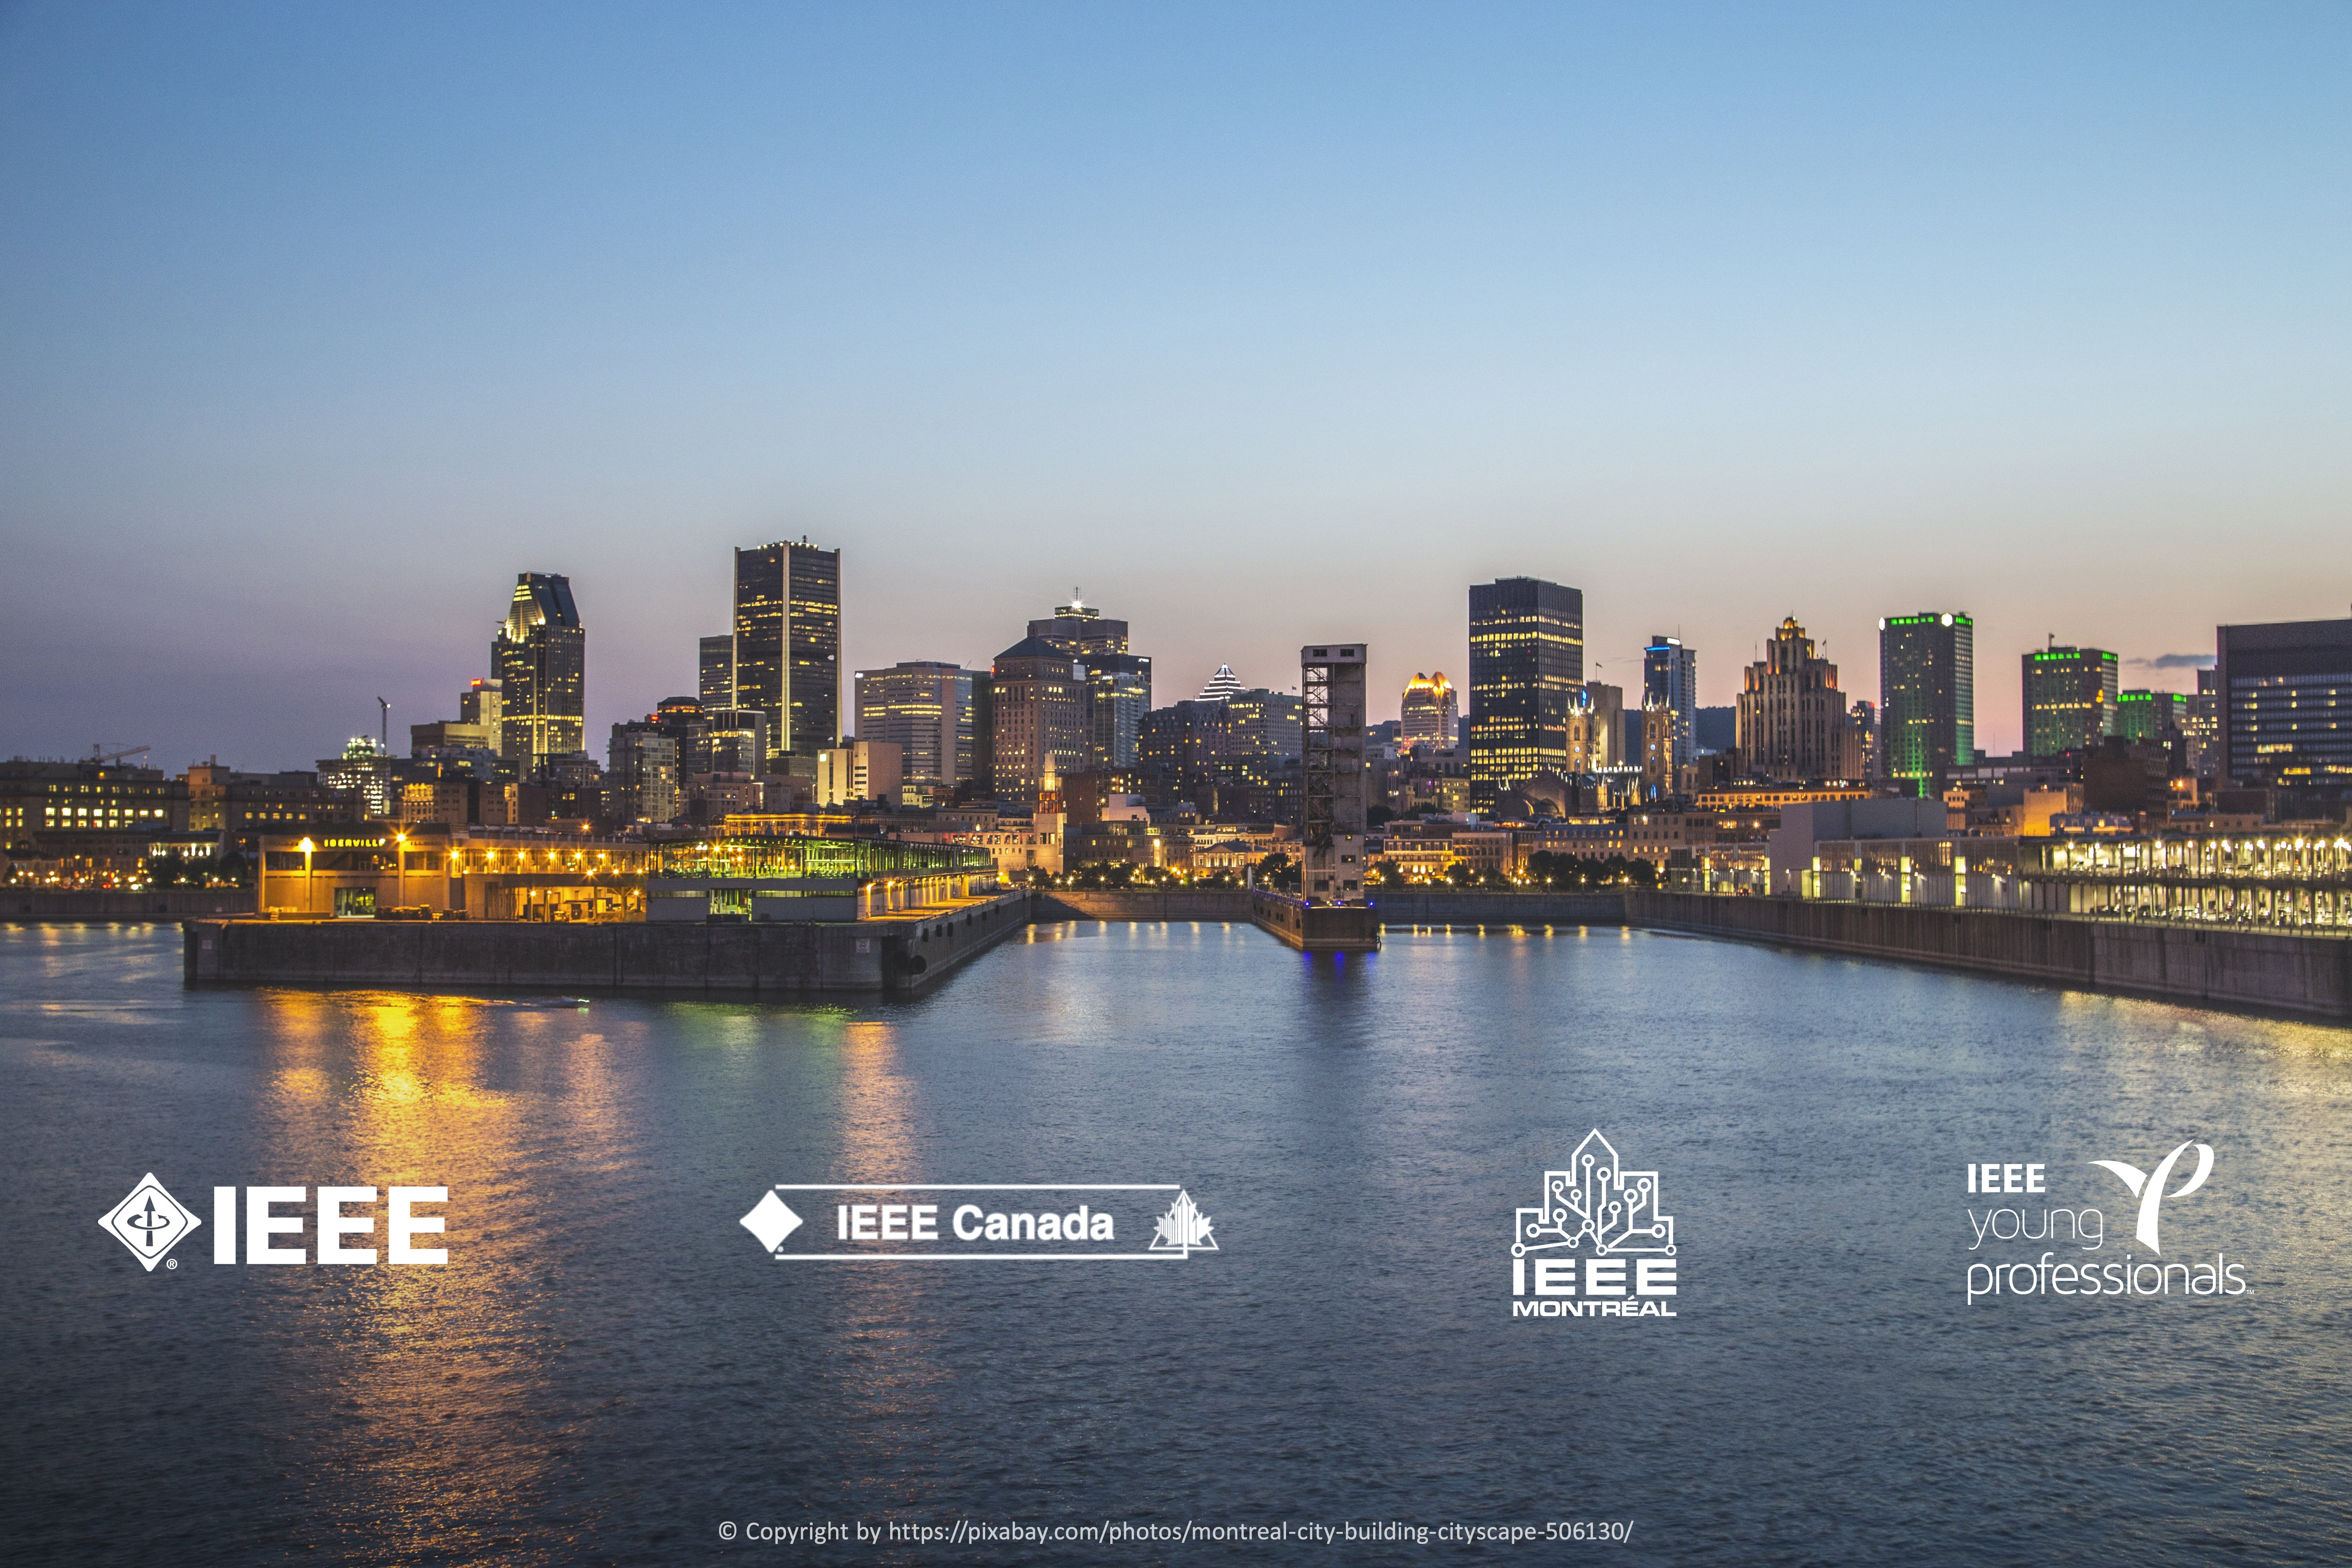
\includegraphics[width=.5\linewidth]{OldPort.jpg}
%	\caption{Old Port}
%	\label{fig:oldport}
%\end{figure}
%
%\begin{figure}
%	\centering
%	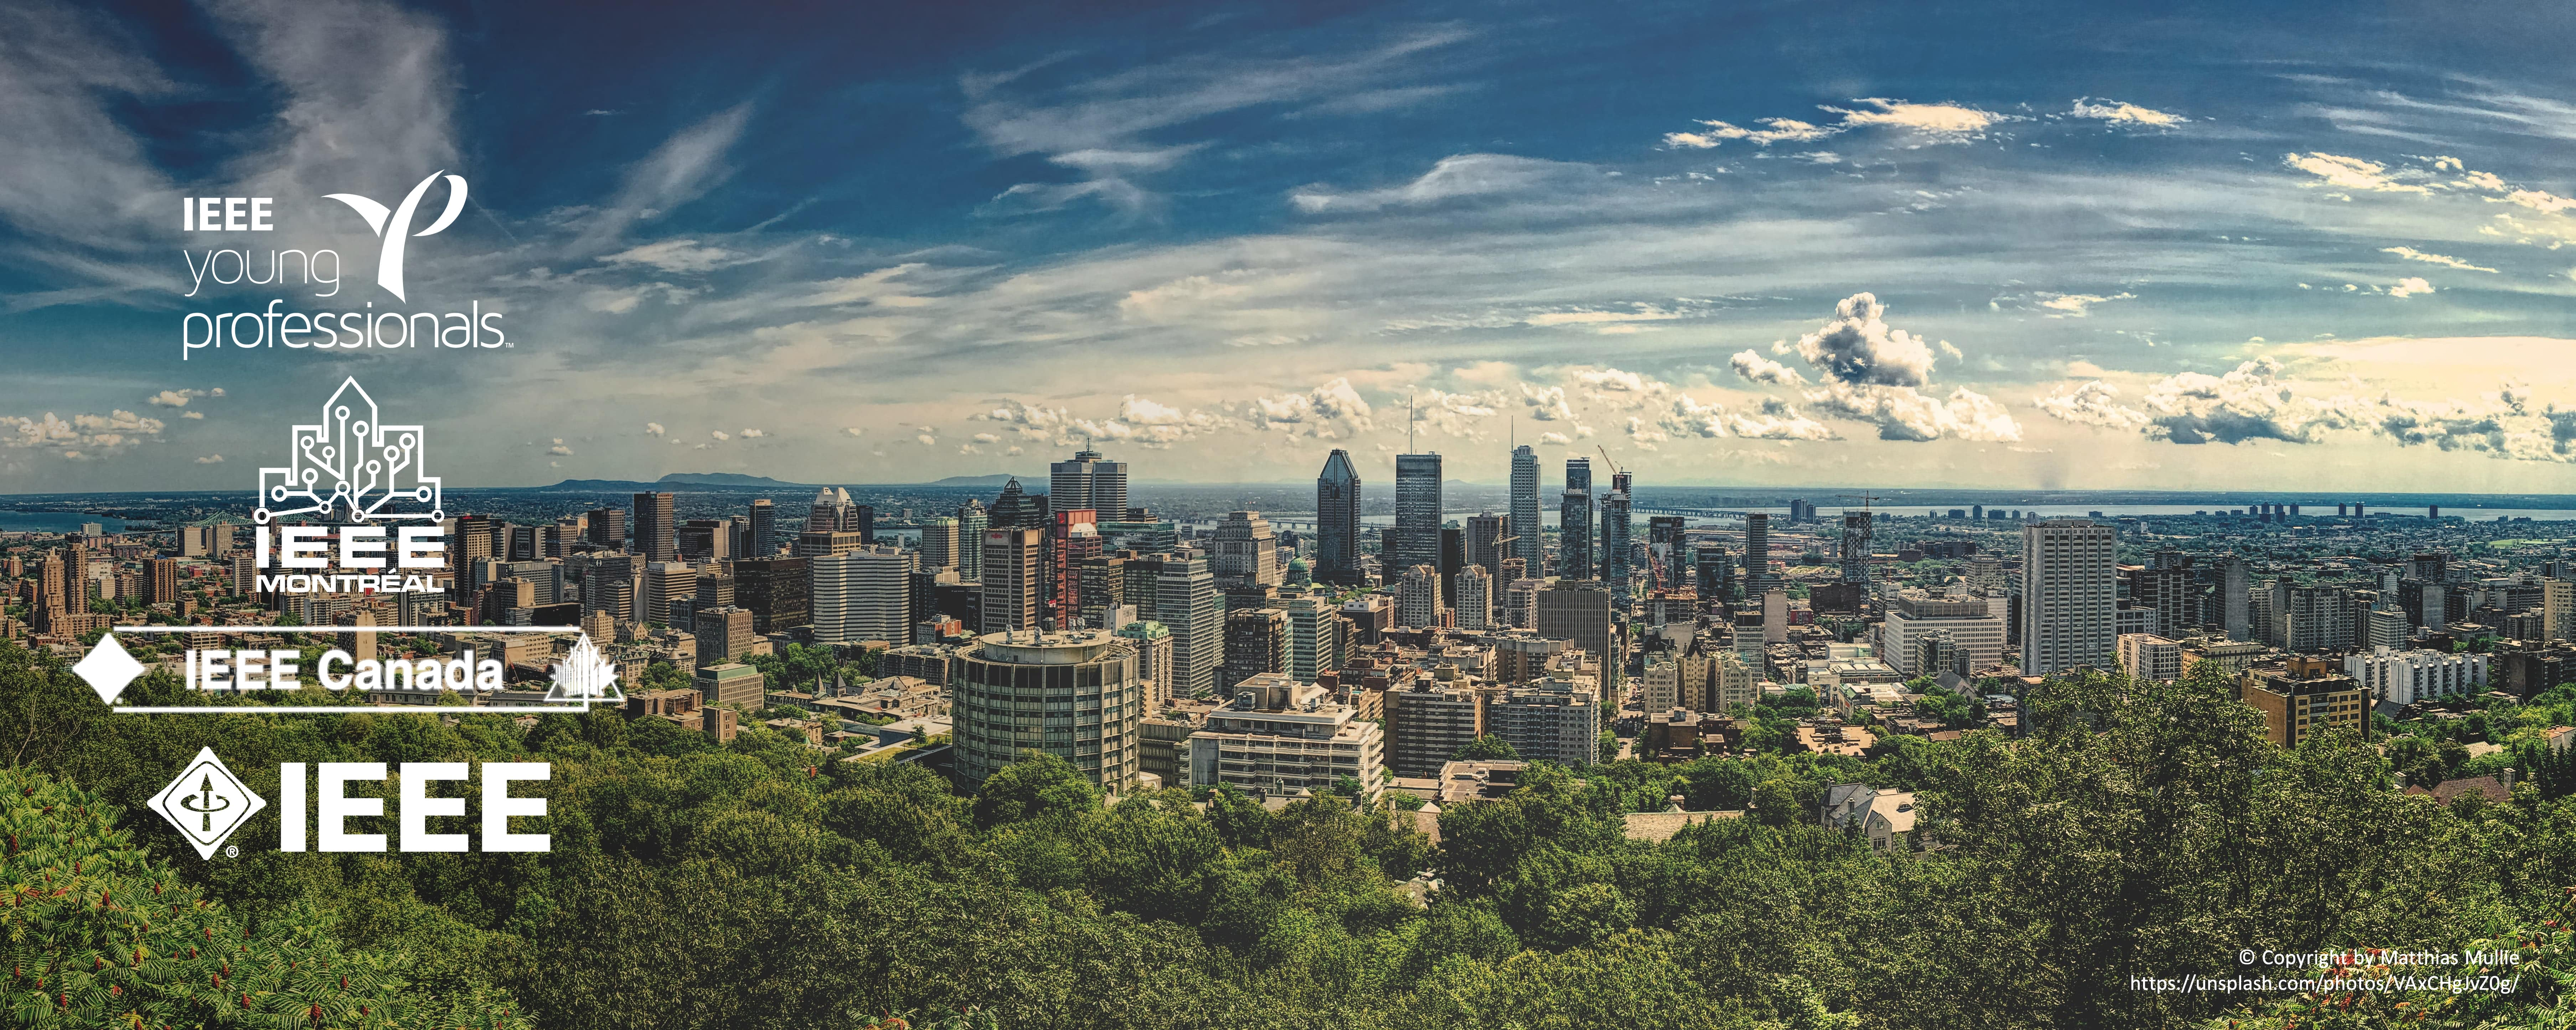
\includegraphics[width=.5\linewidth]{Matthias.jpg}
%	\caption{Mont-Royal}
%		\label{fig:Mont-Royal}
%\end{figure}


I would like to call figure like this. Fig. \ref{fig:oldport}. Now, how to deal with the subfigures. 

\section{Bibliography and Citations}
First, you need to create a bib file. Then, you put your bibtex inside it. Further, you need to call it before \verb|\end{document}|. Let us call the reference \cite{my-paper}. 
	
	
	
	
	
	
	
	
\bibliography{ref}
\bibliographystyle{plain}

	
\end{document}